\section{Approach}

{\bf{Inference in Fully Connected CRFs: }} We briefly review the efficient inference in fully connected CRFs, and refer readers to \citep{krahenbuhl2011efficient} for more details. 

The CRF distribution over pixels is defined as follows.
\begin{align}
  P(\boldsymbol{x}) = \frac{1}{Z} \exp \Big(-E(\boldsymbol{x})\Big)
\end{align}
where $\boldsymbol{x}$ is the label assignment for pixels, and $E(\boldsymbol{x})$ is the energy function. In our experiments, the energy function is
\begin{align}
  E(\boldsymbol{x}) = \sum_i \theta_i(x_i) + \sum_{ij} \theta_{ij}(x_i, x_j)
\end{align}
where the unary potential $\theta_i(x_i) = - \log P(x_i)$, $P(x_i)$ is the probability of assigning label to pixel $i$ (this probability is computed by DCNN), and the pairwise potential $\theta_{ij}(x_i, x_j) = \sum_{m=1}^{K} w^m \cdot k^m(\boldsymbol{f}_i, \boldsymbol{f}_j)$. The edge set is the fully connected edges between any $i$ and $j$, and each $k^m$ is the Gaussian kernel depends on features extracted for piexl $i$ and $j$ and is weighted by parameter $w^m$. We employ the bilateral filtering, which define the kernels as 
\begin{align}
  \theta_{ij}(x_i, x_j) = w^1 \exp \Big(-\frac{|p_i-p_j|^2}{2\sigma_\alpha^2} -\frac{|I_i-I_j|^2}{2\sigma_\beta^2} \Big) + w^2 \exp \Big(-\frac{|p_i-p_j|^2}{2\sigma_\gamma^2}\Big)
\end{align}
where the first kernel depends on both pixel positions (denoted as $p$) and pixel color intensities (denoted as $I$), and the second kernel only depends on pixel positions. The hyper parameters $\sigma_\alpha$, $\sigma_\beta$ and $\sigma_\gamma$ control the ``nearness'' of the Gaussian kernels.

The efficient inference algorithm is based on mean field approximation to the CRF distribution, which finds another simple distribution $b(\boldsymbol{x}) = \prod_i b_i(x_i)$ that minimizes the KL-divergence $KL(b(\boldsymbol{x}) \| P(\boldsymbol{x}))$. The resulting algorithm is stated in \figref{fig:InferenceCRF}. Within the while loop, the first step (\ie, the message passing step) can be expressed as a convolution with a Gaussian kernel in feature space. High-dimensional filtering algorihtms \citep{adams2010fast} have been proposed to speed-up this computation.

\begin{figure}[t]
%\vspace{-0.5cm}
\fbox{
\begin{minipage}[c]{13.5cm}
{\bf Algorithm: Efficient Inference in Fully Connected CRFs}

Initialize $b_i(x_i) \leftarrow \frac{1}{Z_i} \exp \Big(-\theta_i(x)i \Big)$

{\bf While} not convergenced, 

\begin{enumerate}[labelindent=0pt,labelwidth=\widthof{\ref{last-item}},label=\arabic*.,itemindent=2em,leftmargin=0pt]
\item $\tilde{b_i}^m(l) \leftarrow \sum_{j \neq i}k^m(\boldsymbol{f}_i,\boldsymbol{f}_j) \cdot b_j(l), \ \forall m$
\item $\hat{b_i}(x_i) \leftarrow \sum_{l} \sum_m w^m \cdot \tilde{b_i}(l)$
\item $b_i(x_i) \propto \exp \Big(-\theta_i(x_i) - \hat{b_i}(x_i) \Big)$
\end{enumerate}

\end{minipage}
}
\caption{Efficient Inference algorithm in Fully Connected CRFs
}
\label{fig:InferenceCRF}
\end{figure}



\begin{figure}
  \centering
  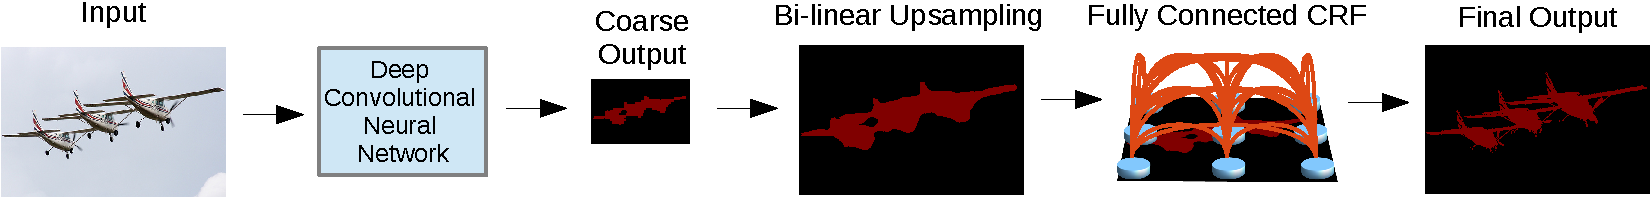
\includegraphics[width=1\linewidth]{fig/model_illustration.pdf}
  \caption{Model Illustration. The coarse output of Deep Convolutional Neural Network (with fully convolutional layers) is upsampled by bi-linear interpolation. A fully connected CRF is applied to refine the segmentation result.}
  \label{fig:ModelIllustration}
\end{figure}




 

